\begin{figure}[t]
\centering
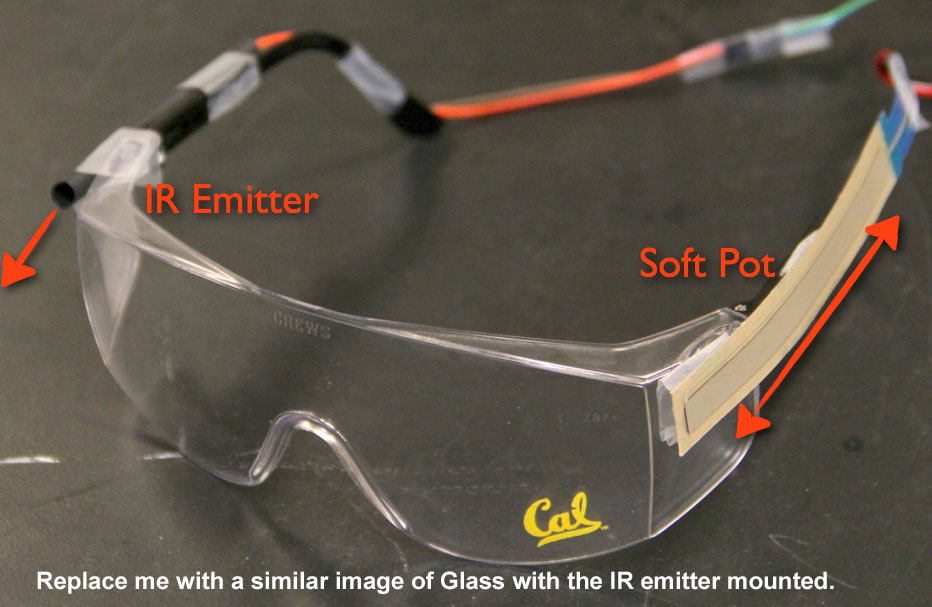
\includegraphics[width=1.0\columnwidth]{figures/glass-with-ir}
\caption{Our augmented Glass prototype has a frame-mounted infrared emitter.}
\label{fig:glass}
\end{figure}
\begin{figure}[t]
\centering
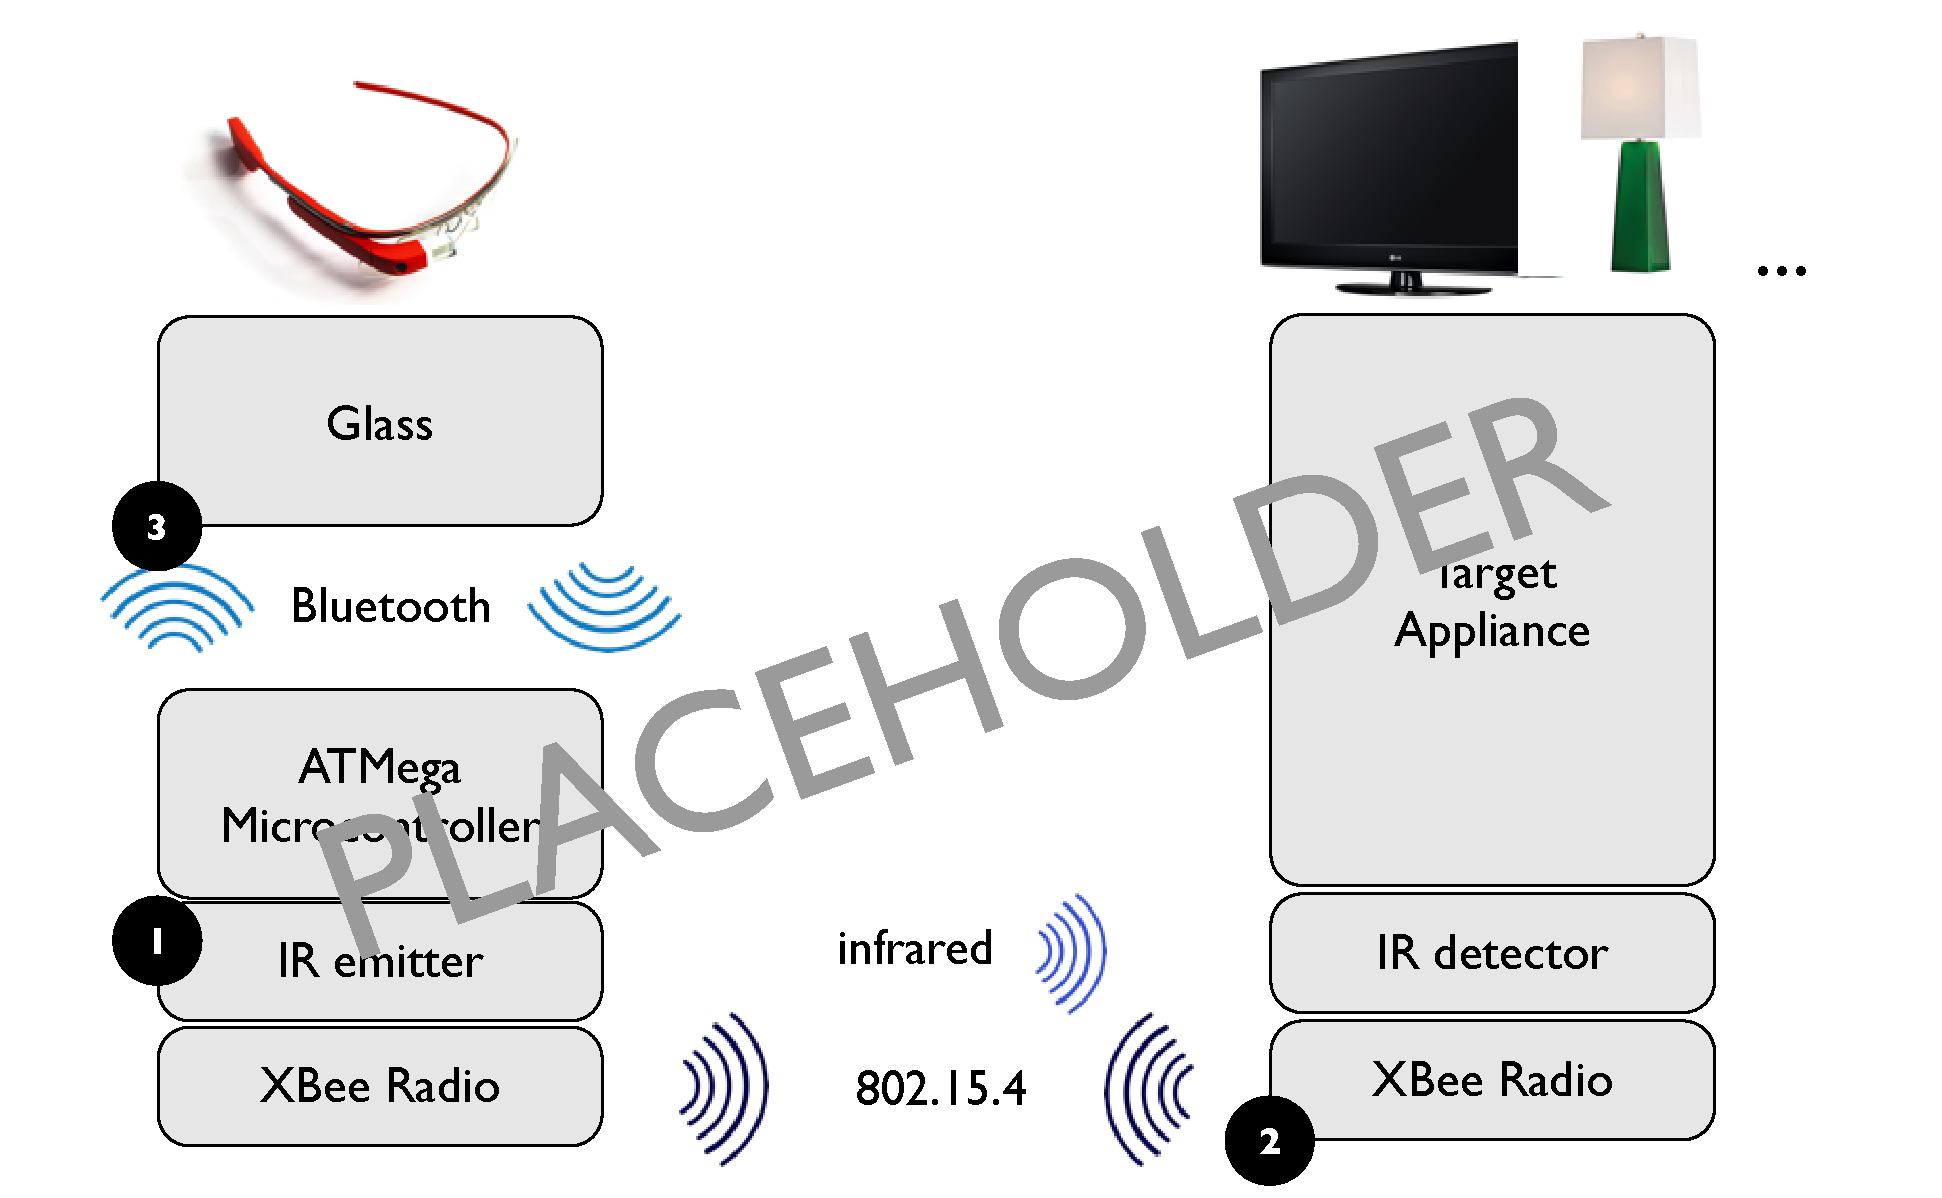
\includegraphics[width=1.0\columnwidth]{figures/architecture}
\caption{System architecture.}
\label{fig:architecture}
\end{figure}

\section{Interaction and Hardware Device}

\subsection{Design Goals}
{\bf Leverage visual attention:} Take advantage of the fact that visual attention can express intention - trigger interaction based on where a user is already looking

{\bf Provide feedback in the environment:} While a near-eye display can push information to the user, locate visual feedback about selection targets in the environment, to prevent distraction and interruption.

{\bf Deal with dense device arrangements and the limit of head positioning}

\bjoern{Finish and expand this section.}

\subsection{Interaction Flow}
{\bf Look:} Users select a target device by looking in its general direction.
Glass periodically sends a device id through its IR emitter analogous to Patel's approach~\cite{patel_2-way_2003}. Target appliances have IR receivers and offer immediate visual feedback by toggling a red LED whenever a valid id is received. This enables {\em scanning} the environment with ones gaze to see which devices can be controlled. They also respond by initiating an XBee radio connection and sending their id. This allows the Glass application to show which devices are currently targeted on the display. \sean{Currently the led is implemented but clients don't response with their IDs and display on Glass at this stage. We can add that. But we felt like the users would use led as the primary indicator and not to distract them with frequently changing the content on the screen? }

{\bf Initiate:} Users confirm to initiate interaction by tapping on the Glass touchpad. The next section on disambiguation deals with cases in which multiple devices received valid IR signals. At this point, all further communication switches over to the XBee wireless network so that line of sight to the target is no longer needed (otherwise restricting head movement can become straining).

{\bf Control:} Glass displays a control interface for parameters of the chosen device. \bjoern{Describe the interaction scheme for navigating and adjusting parameters here}.
Control commands are sent over XBee radios.

{\bf Disengagement:} \bjoern{how do you end an interaction? Is there a timeout if the user forgets to manually back out of the control screen?} \sean{currently the only way is to swipe back. A timeout mechanism can be added easily. I guess the design decision lies in what is an appropriate duration?}

\subsection{Disambiguation}
\bjoern{describe why disambiguation is necessary - combination of the relative inaccuracy of head orientation and the spread of our IR signal. Then describe how to overcome it.}

\subsection{Prototype Implementation}
Our prototype consists of a Google Glass Explorer Edition head-worn computing device, augmented with an infrared emitter that is mounted on the frame, pointing out in the direction of the wearer's view (Figure~\ref{fig:glass}). The IR emitter LED is mounted in an opaque hollow tube, that restricts the outgoing angle of illumination. 

In our prototype, Glass communicates over Bluetooth to an additional microcontroller board the user has to wear (Atmel ATMega256). This board marshals XBee to Bluetooth messages in both directions and also controls the IR LED mounted on the Glass frame (Figure~\ref{fig:architecture}). This architecture was mostly chosen for reasons of expediency. We selected XBee 802.15.4 radios to avoid the latency associated with connecting and disconnecting to Bluetooth devices \bjoern{Is this true or not?} \sean{Origainlly we didn't know we'd work on Google Glass, therefore BT didn't have a higher priority. We learned that bluetooth can concurrently communicate with up to 7 devices (while up to 255 can be paired but inactive), giving us more complexity when scaling up. In addition ZigBee has shorter wakeup delay and lower power consumption. (referenced here: http://superuser.com/questions/332767/limit-to-the-number-of-devices-that-can-be-paired-with-a-bluetooth-device)} Future head-mounted devices could clearly integrate IR emitters; the choice of local wireless technology could also change. In particular, one could substitute WiFi modules. 

\section{Device Characterization}
We determined the usable range and accuracy empirically with one IR emitter and two IR receivers. The IR emitter constantly sent out an id signal. The receivers that correctly received the signal turn their LED on for 300 ms.

We placed all three devices at the same height with clear line of sight. The IR emitter is first places 2 feet away from the receivers. The receivers were moved sideways apart from each other until they could no longer receive stable signals. We then recorded the distance of the two receivers for the calculation of coverage angles. The steps are repeated for IR emitters in different distances (as shown in Table~\ref{table:measurements}). We then repeated measurements with the emitter  placed at various depths in the tube (see Figure~\ref{fig:coverage}). 

In summary, \bjoern{describe what the measured results mean in practice.}

\begin{figure}[t]
\centering
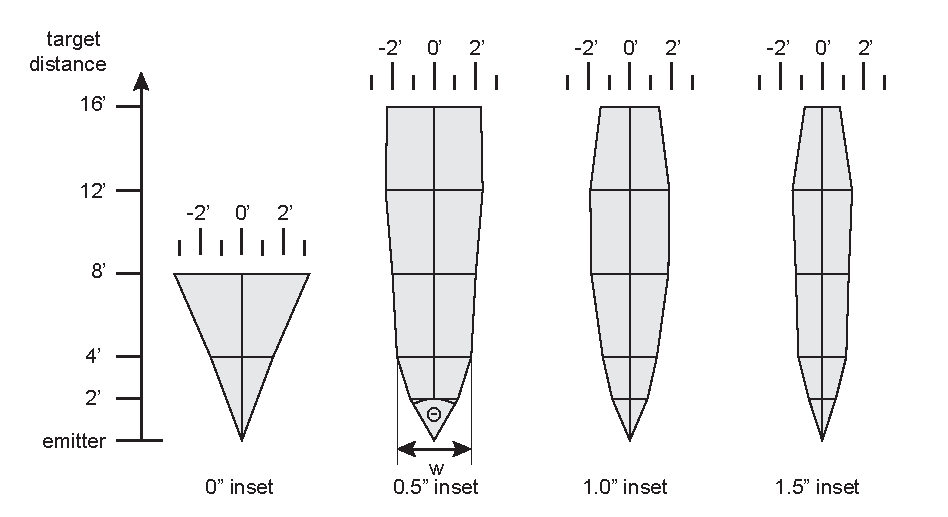
\includegraphics[width=1.0\columnwidth]{figures/glass-ir-coverage}
\caption{Different IR configurations suggest that usable beam widths of 2 to 4 feet and distances up to 16 feet }
\label{fig:coverage}
\end{figure}

\begin{table}
    \begin{tabular}{l|lllll}
    distance/ depth & \ft2       & \ft4       & \ft8   & \ft{12}  & \ft{16}  \\ \hline
    \inch{0}                     & $74\degree$ & $78\degree$ & N/A  & N/A  & N/A  \\
  \inch{0.5}                   & $60\degree$ & $48\degree$     & $28\degree$ & $22\degree$ & $16\degree$ \\
    \inch{1.0}                     & $46\degree$     & $36\degree$     & $26\degree$ & $18\degree$ & $10\degree$ \\
    \inch{1.5}                   & $36\degree$     & $32\degree$     & $18\degree$ & $14\degree$ & $6\degree$  \\
    \end{tabular}
    \caption{Measured IR coverage angles $\Theta$ at different target distances and different depths of IR emitter inside shielding tube.}
    \label{table:measurements}
    
\end{table}